% 
% Annual Cognitive Science Conference
% Sample LaTeX Paper -- Proceedings Format
% 

% Original : Ashwin Ram (ashwin@cc.gatech.edu)       04/01/1994
% Modified : Johanna Moore (jmoore@cs.pitt.edu)      03/17/1995
% Modified : David Noelle (noelle@ucsd.edu)          03/15/1996
% Modified : Pat Langley (langley@cs.stanford.edu)   01/26/1997
% Latex2e corrections by Ramin Charles Nakisa        01/28/1997 
% Modified : Tina Eliassi-Rad (eliassi@cs.wisc.edu)  01/31/1998
% Modified : Trisha Yannuzzi (trisha@ircs.upenn.edu) 12/28/1999 (in process)
% Modified : Mary Ellen Foster (M.E.Foster@ed.ac.uk) 12/11/2000
% Modified : Ken Forbus                              01/23/2004
% Modified : Eli M. Silk (esilk@pitt.edu)            05/24/2005
% Modified : Niels Taatgen (taatgen@cmu.edu)         10/24/2006
% Modified : David Noelle (dnoelle@ucmerced.edu)     11/19/2014

%% Change "letterpaper" in the following line to "a4paper" if you must.

\documentclass[10pt,letterpaper]{article}

\usepackage{cogsci}
\usepackage{pslatex}
\usepackage{apacite}
\usepackage{subcaption}
\usepackage{todonotes}
\usepackage{amsmath}

%% commands
\newcommand{\set}[1]{\left\{#1\right\}}
\DeclareMathOperator{\expo}{exp}
\newcommand{\citet}[1]{\citeA{#1}}
\newcommand{\citep}[1]{\cite{#1}}


\title{What does the crowd believe? A hierarchical approach to estimating subjective beliefs
  from empirical data}
 
\author{{\large \bf Erin Bennett, Judith Degen, Michael Henry Tessler, Noah D. Goodman}\\
     \{ebennett,jdegen,mhtessler,ngoodman\}@stanford.edu \\
     Department of Psychology, 450 Serra Mall \\
  Stanford, CA 94305 USA \AND {\large \bf Michael Franke} \\
  michael.franke@uni-tuebingen.de \\
  Department of Linguistics, Wilhelmstra\ss e 19 \\
 72074 T\"{u}bingen, Germany
  \AND}


\begin{document}

\maketitle

\todo[inline]{Each author's name should appear
on a separate line, 11~point bold, and centered, with the author's
email address in parentheses. Under each author's name list the
author's affiliation and postal address in ordinary 10~point type.}

\todo[inline]{who is an author? which order?}


\begin{abstract}
  Subjects' beliefs about everyday events are of theoretical interest on their own and also an
  important ingredient in especially Bayesian models of such diverse phenomena as logical
  reasoning, future predictions or language use and interpretation. Here, we scrutinize one
  recently popular method for measuring subjective beliefs experimentally. We present a
  hierarchical Bayesian model for inferring likely ``population-level beliefs'' as the central
  tendency of subjects' individual-level beliefs. Individual-level beliefs define likelihood
  functions for three types of task measures. Our results suggest that the previous practice of
  using averaged normalized slider ratings for binned quantities is a practical and fairly good
  approximator of latently inferred population-level beliefs.

\textbf{Keywords:} subjective beliefs, hierarchical modeling, Bayesian data analysis, Bayesian
cognitive models 
\end{abstract}




\section{Motivation}

We cannot look into a person's head. But in making sense of observed behavior we readily
ascribe beliefs and desires to fellow agents. This happens intuitively, in folk psychology, but
also in science. Ascriptions of latent mental states play an important role as well in many
explanations of especially higher-order cognition, like decision making, planning, reasoning,
or language use. Naturally, then, it becomes important how to validate any putative ascription
of mental states for explanatory purposes.

A family of models where this is particularly pressing are Bayesian models of cognition which
seek to explain task behavior in a variety of domains as partially informed by what subjects
believe about mundane events. Take interpretation of language. Empirical data on whether a
statement like ``That watch cost $n$ dollars'' is understood to convey speaker affect, rather
than literal meaning, can be explained well by a Bayesian model of utterance interpretation
\citep{KaoWu2014:Nonliteral-Unde} in which a crucial role is played, as is quite intuitive, by
an empirical measure of subjects' expectations about the likely or normal price of a
watch. Other examples of domains in which empirically successful models have included some
measure of subjects' belief include making future predictions
\citep{GriffithsTenenbaum2006:Optimal-Predict}, the strength of pragmatic enrichments
\citep{DegenTessler2015:Wonky-worlds:-L}, the interpretation of vague quantifiers
\citep{SchollerFranke2015:Semantic-values}, \textcolor{red}{ \dots }

\todo[inline]{fill me}

Many methods of assessing subjective beliefs exist. One approach is to take actual frequencies
as an approximation \citep{GriffithsTenenbaum2006:Optimal-Predict}. This, however, does not
work for beliefs about one-shot or imaginary events. Moreover, even where available, real-world
frequencies may deviate systematically from subjects' beliefs, and this can be problematic for
the predictions of a model that relies on subjective beliefs
\citep{MarcusDavis2013:How-Robust-Are-}.

Another approach is to try to experimentally measure relevant beliefs. Many techniques for this
exist, especially in the economics literature
\citep{MorganHenrion1990:Uncertainty:-A-,Manski2004:Measuring-Expec,SchlagTremewan2014:A-penny-for-you,AndersenFountain2014:Estimating-Subj}. The
perhaps most prominent method uses so-called \emph{scoring rules}
\citep{Savage1971:Elicitation-of-,SchlagTremewan2014:A-penny-for-you}. Roughly speaking,
scoring rules are particular schemes of rewarding participants' answers in such a way as to
make sure that responses are what we want them to be: the actual subjective probability of an
event, the mean of a distribution, a credible interval etc. Scoring rules are highly faithful
but require participants to become sufficiently familiar with the (usually probabilistic)
payoff scheme. Scoring rules also must make assumptions about how much participants value
certain probabilistic gambles and may therefore require elaborate means of data analysis
\citep{AndersenFountain2014:Estimating-Subj}. Similar practical concerns apply to other methods
as well, such as the use of \emph{iterated learning} for prior estimation
\citep{LewandowskyGriffiths2009:The-Wisdom-of-I}.

For common applications, many of these procedures may be excessively complex or too demanding
on both researcher and participant. It would be beneficial if there was an easily applicable
technique of eliciting subjective beliefs that is good enough for testing the general
predictions of models that rely on these measures for their predictions. A further complication
is that it may be impractical to obtain, from the same participant, data on subjective beliefs
and data on the task of interest, especially if exposure to one of these measures is likely to
affect the other. This suggests that, for practical reasons, there is a demand of
reliable-enough measures of what we will sloppily call ``population-level beliefs'': estimates
of the central tendency or average of subjective beliefs in a given population.

A very simple technique that has been used with apparent success is to have subjects adjust
sliders in order to express their (relative) levels of support for values of uncertain
contiguous quantities
\citep{KaoWu2014:Nonliteral-Unde,SchollerFranke2015:Semantic-values}. \textcolor{red}{ MORE REFERENCES } Subjects are confronted with a short and simple description of a situation or an
event, such as ``John bought a watch,'' and asked for their estimates of the watch's price. To
give their estimate, they are asked to adjust sliders, whose ends are labelled as ``extremely
likely'' and ``extremely unlikely,'' for a number of bins that partition the range of plausible
values (established by a pre-test). E.g., for the price of a watch bins could be
\textcolor{red}{ FILL ME }

\begin{itemize}
\item explain slider rating task
\item our goal here is to validate whether ``population-level beliefs'' are approximated well
  enough by normalized average slider ratings
\item use hierarchical Bayesian modeling
  \begin{itemize}
  \item calculate likelihoods from subjective beliefs
  \item each subjective belief is drawn from a population-level central tendency, which is a
    ``belief'' as well
  \end{itemize}
\end{itemize}

\section{Experiments}

\begin{itemize}
\item why within-participant?
\item what was the exact randomization / procedure?
\item items are given in Table~\ref{tab:Items}
\item include bins as well?
\item what were the lighting round bin comparisons?
  \begin{itemize}
  \item 1 vs 2
  \item 2 vs 6
  \item 6 vs 11
  \item 11 vs 14
  \item 14 vs 15
  \end{itemize}
\item results are in Figure~\ref{fig:Results}
\end{itemize}

\begin{table}
  \centering
  \begin{tabular}{p{8cm}}
    1.  X has just fetched himself a cup of \textbf{coffee} from the office vending machine.
         What do you think the temperature of his coffee is?  \\
    2.  X \textbf{commuted} to work yesterday. 
        How many minutes do you think she spent commuting yesterday? \\
3.  X told a \textbf{joke} to N kids. 
    How many of the kids do you think laughed?\\
    
4.  X bought a \textbf{laptop}.    
    How much do you think it cost?\\
    
5.  X threw N \textbf{marbles} into a pool.
    How many of the marbles do you think sank?\\

6.  X just went to the \textbf{movies} to see a blockbuster.
    How many minutes long do you think the movie was?\\

7.  X watched \textbf{TV} last week.
    How many hours do you think he spent watching TV last week? \\

8.  X bought a \textbf{watch}.
    How much do you think it cost?
  \end{tabular}
  \caption{Experimental items}
  \label{tab:Items}
\end{table}

\begin{figure}
  \centering
  \begin{subfigure}[b]{0.5\textwidth}
    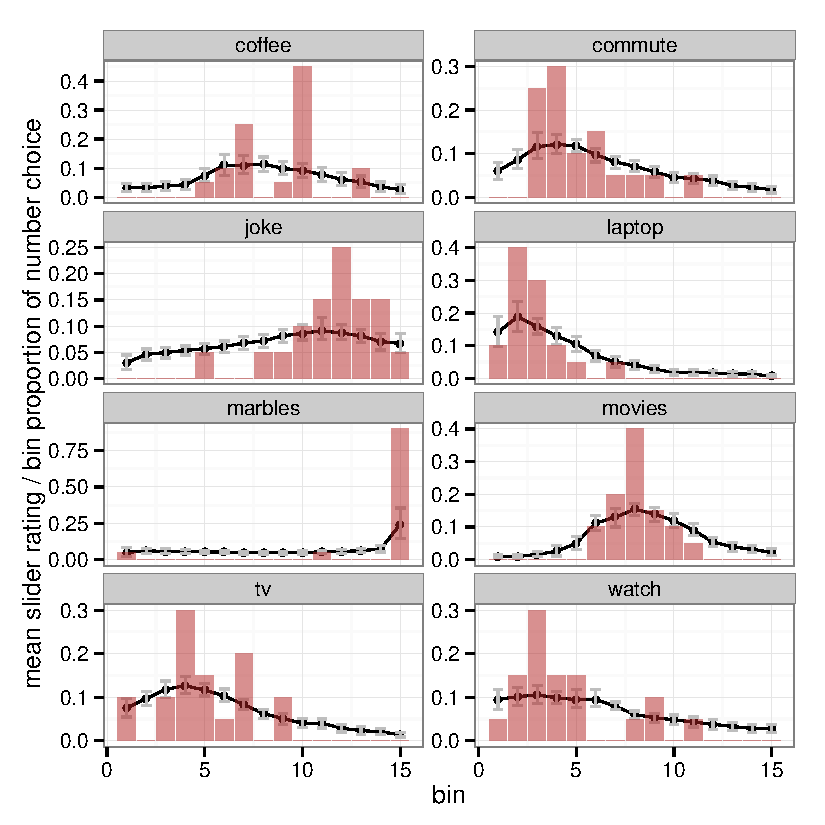
\includegraphics[width = \textwidth]{plots/data_sliderNumber.pdf}
    \caption{slider ratings \& number choices}
    \label{fig:slider}
  \end{subfigure}

  \begin{subfigure}[b]{0.5\textwidth}
    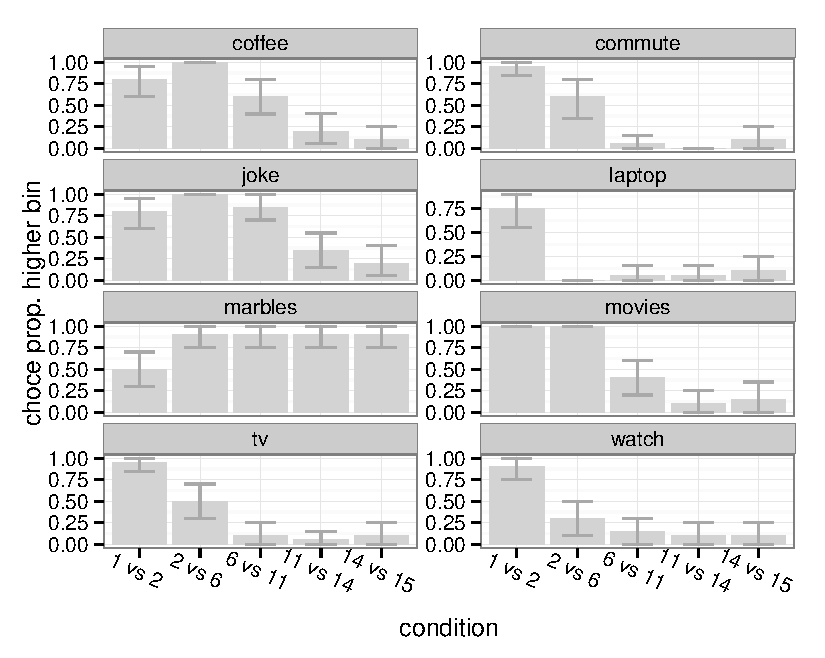
\includegraphics[width = \textwidth]{plots/data_choice.pdf}
    \caption{bin comparison}
    \label{fig:lighting}
  \end{subfigure}

  \caption{Results from experiments. Error bars show bootstrapped 95\% confidence intervals.}
  \label{fig:Results}
\end{figure}


\section{Model}

The data we would like to explain are: (i) the normalized slider ratings $s_{ijk} \in [0;1]$ of
subject $i \in \set{1, \dots, 20}$ for item $j \in \set{1, \dots, 8}$ and bin
$k \in \set{1, \dots, 15}$; (ii) the bins $n_{ij} \in \set{1, \dots, 15}$ in which subject
$i$'s number choice for item $i$ was; and (iii) the binary choices $c_{ijl} \in \set{0,1}$ of
whether subject $i$ selected the higher bin for item $j$ in the bin comparison condition
$l$. There two simplifications in need of commenting. In (i), we focus on slider ratings after
normalizing for each subject, because we assume that slider adjustments reflect relative, not
absolute estimates of subjective beliefs. In (ii), we focus on bin choices, not actual number
choices, in order to avoid, as much as possible, considerations of salience of particular
numbers, and also because otherwise data from items with smaller domains of plausible number
would get more weight than data from items which allow for a wider set of number choices.

All three pieces of data are to be explained as functions of subjective beliefs $P_{ij}$, where
$P_{ij}$ is a probability vector of length 15 with $P_{ijk}$ being subject $i$'s belief about
the relative likelihood of bin $k$ for item $j$. Each $P_{ij}$ defines a likelihood for our
data, via appropriate link functions (to be spelled out presently). Variance in subjective
beliefs is harnessed by a population-level hyper-prior with central tendency $Q_{j}$, i.e., a
stochastic vector of length 15, which we call a ``population-level belief'' about item $j$. The
structure of this model is pictured in Figure~\ref{fig:ModelGraph}.

\begin{figure}[]
  \centering
  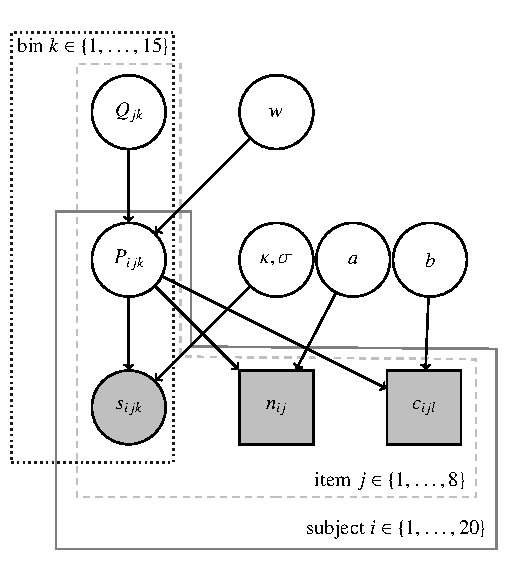
\includegraphics[width = 0.4\textwidth]{modelGraph/modelGraphNoMath.pdf}
  \caption{The data-generating model as a probabilistic graphical model, following conventions
    of \citet{LeeWagenmakers2013:Bayesian-Cognit}. Shaded nodes are observed, white nodes are
    latent variables. Square nodes represent categorical, round nodes continuous
    variables. Boxes indicate scope of indices.}
  \label{fig:ModelGraph}
\end{figure}

To fill the structure in Figure~\ref{fig:ModelGraph} with life, we need to spell out three
parameterized link functions, one for each task type, and the relation between population-level
belief $Q_j$ to individual beliefs $P_{ij}$. Let's start with the latter. For fixed $Q_j$, the
idea is that $P_{ij}$ are noise-perturbed variants scattered around $Q_j$, with some parameter
$w$ to determine how much perturbation we should expect. To realize this, the model assumes
that $P_{ij}$ are distributed according to a Dirichlet distribution with weights given by
$w Q_{j}$:
\begin{align*}
  Q_j & \sim \text{Dirichlet}(1, \dots, 1) & w & \sim \text{Gamma}(2,0.1) \\
  P_{ij} & \sim \text{Dirichlet}( w Q_j)
\end{align*}
The higher $w$, the more likely it is that $P_{ij}$ is ``close'' to $Q_j$.

The link function for the slider rating data uses a logit transformation to project observed
slider ratings $s_{ijk}$ and latent probabilities $P_{ijk}$, which are bound to lie between 0
and 1, to the reals. The likelihood of logit-transformed observation $s_{ijk}$ is given by a
Gaussian with standard deviation $\sigma$ around the logit-transformed predictor $P_{ijk}$. On
top of that, there is a parameter $\kappa$, the steepness of the logit transform of $P_{ijk}$,
that allows response likelihoods to capture end-point affinity for $\kappa >1$ (values of
$P_{ijk}$ close to 0 or 1 are likely mapped to 0 or 1) or end-point aversion for $\kappa <0$
(values of $P_{ijk}$ are likely to be realized as more median), with a prior that expects
$\kappa=1$.
\begin{align*}
  \text{logit}(s_{ijk}) &\sim
        \text{Norm}(\text{logit}(P_{ijk}, \kappa), \sigma) \\
        \sigma &  \sim \text{Gamma}(0.0001,0.0001) & \kappa &\sim \text{Gamma}(5,5)
\end{align*}
 
The link function for number choice data treats each bin $n_{ij}$ as a draw from a categorical
distribution where the probability of bin $k$ is proportional to $\expo(a P_{ij})$, i.e., a
soft-max choice from $P_{ij}$. The higher parameter $a$, the more likely $n_{ij}$ is the mode
of $P_{ij}$. For $a \rightarrow 0$, all bins become equiprobable.
\begin{align*}
  n_{ij} & \sim
        \text{Categorical}(\expo(a P_{ij})) &
 a & \sim \text{Gamma}(2,1)
\end{align*}

Finally, consider the link function for bin comparisons. We are after the likelihood with which
subject $i$ selects the higher bin for item $j$ in bin comparison condition $l$. Suppose $l$ is
about comparing the lower bin $b_l$ to the higher $b_h$. The perhaps most natural approach
would be to link the likelihood of choosing $b_h$ over $b_l$ to the difference between
$P_{ijb_h}$ and $P_{ijb_l}$. This, however, does not appear to be what subjects were doing. For
example, take the ``marbles'' case where we see almost unanimous choices of bin 11 over bin 6,
despite seeing any pronounced difference in slider ratings for these bins. Indeed, a model that
implements this idea failed to capture the relevant regularities in the data blatantly.

Another plausible link function that accommodates for this is to assume that what matters in
bin comparisons is the distance to the mode of $P_{ij}$: soft-max prefer the bin that is closer
to the mode of $P_{ij}$; select random if both bins are equally far from the
prototype.\footnote{Notice that
  $(1 + \exp(2b(1-p^{\text{high}}_{ijl})) )^{-1} = \frac{\exp(b p^{\text{high}})}{\exp(b
    p^{\text{high}}) + \exp(b p^{\text{low}})}$
  with $p^\text{low}_{ijl} = 2 - p^\text{high}_{ijl}$.}
\begin{align*}
  c_{ijl} & \sim \text{Bern}( (1 + \exp(2b(1-p^{\text{high}}_{ijl})) )^{-1} ) \ \ \ 
  b  \sim \text{Gamma}(2,1) \\
  p^\text{high}_{ijl} & = \begin{cases}
    2 & \text{if $mode(P_{ij})$ is closer to higher} \\
    & \text{ bin of $l$ than to lower bin } \\ 1 & \text{if equal
      distance} \\ 0 & \text{otherwise}  
  \end{cases}
\end{align*}


\section{Inference}

The model was implemented in JAGS \cite{Plummer2003:JAGS:-A-Program}. 50,000 samples were
obtained from two chains with a thinning rate of 2 after a burn-in of 100,000 that ensured
convergence according to $\hat{R}$ \cite{GelmanRubin1992:Inference-from-}.

Of most theoretical interest are posterior estimates of $Q_j$. Figure~\ref{fig:PosteriorQj}
shows means of the posterior $Q_j$, with their 95\% HDIs, alongside the averaged normalized
slider ratings. The latter provide a very good approximation of the latent, inferred
population-level beliefs. Inspection of posteriors of individual $P_{ij}$ shows that there is
ample variation between subjects. Nonetheless, the way the model suggest we should think about
harnessing the individual $P_{ij}$s under a population-level central tendency is closely
approximated by simply averaging over slider ratings. Although the match is clearly not
perfect, it is good enough to maintain that the latter are a reasonable (enough) and practical
way of assessing what the crowd believes despite individual differences.

\begin{figure}
  \centering
  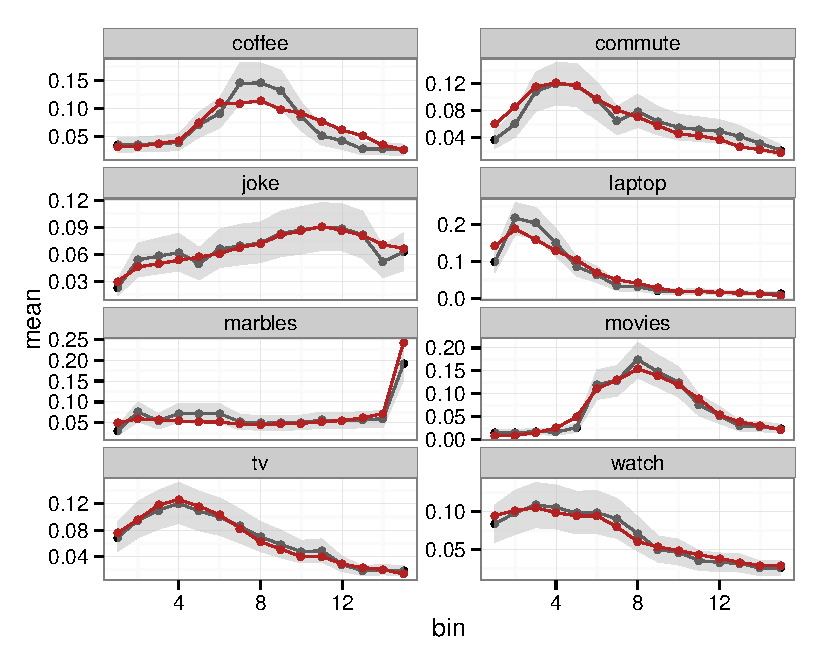
\includegraphics[width = 0.5\textwidth]{plots/pop_priors.pdf}
  \caption{Means of posteriors over $Q_j$ in black with gray area indicating 95\% HDIs. Red
    lines give the average normalized slider ratings for comparison.}
  \label{fig:PosteriorQj}
\end{figure}

\section{Model criticism}

Inferences based on the model are only as reliable as the model itself is plausible. Model
criticism is therefore important. Figure~\ref{fig:PPCs} shows posterior predictive checks at
the population-aggregate level for all of our three task types. For the slider rating task,
posterior predictions are spot-on. Some of the number estimation data is surprising even for
the model trained on this very data. This could have various reasons: (i) the number data does
not have a huge influence on the posterior likelihood, (ii) number choices may be influenced by
saliency and/or roundness of numbers after all. Finally, there is one condition in the bin
comparison task that the model definitely got wrong. This is the choice of what is more likely:
that one or that none of 14 marbles thrown into a pool would sink. The model would predict that
almost everybody should answer that it is more likely that one marble sank. But that is not
what we observe. It may be that subjects revise beliefs about ``normality'' of the marbles,
while holding on to an assumption that all marbles behave the same
\cite{DegenTessler2015:Wonky-worlds:-L}.

\begin{figure}
  \centering
  \begin{subfigure}[b]{0.5\textwidth}
    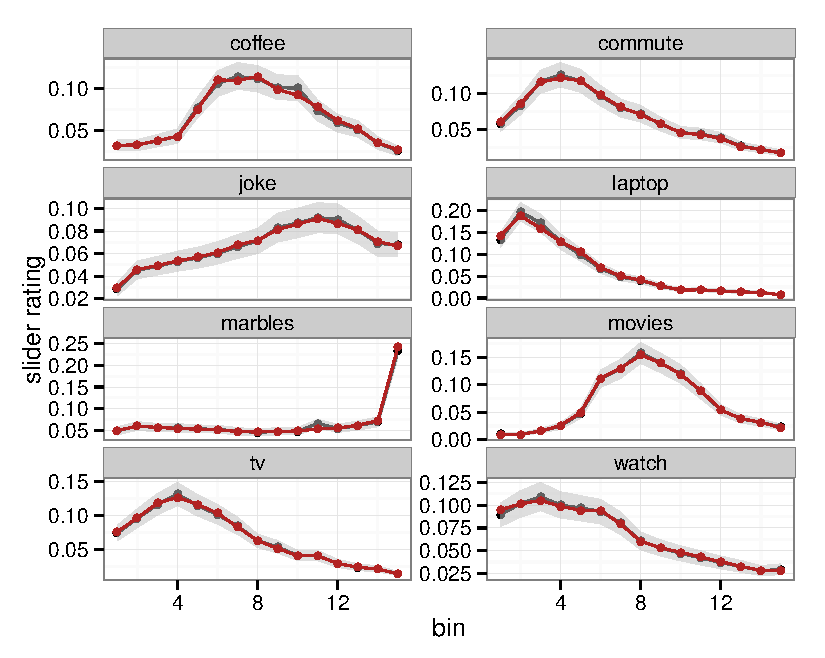
\includegraphics[width = \textwidth]{plots/ppc_slider.pdf}
    \caption{slider rating}
    \label{fig:sliderPPC}
  \end{subfigure}
   
  \begin{subfigure}[b]{0.5\textwidth}
    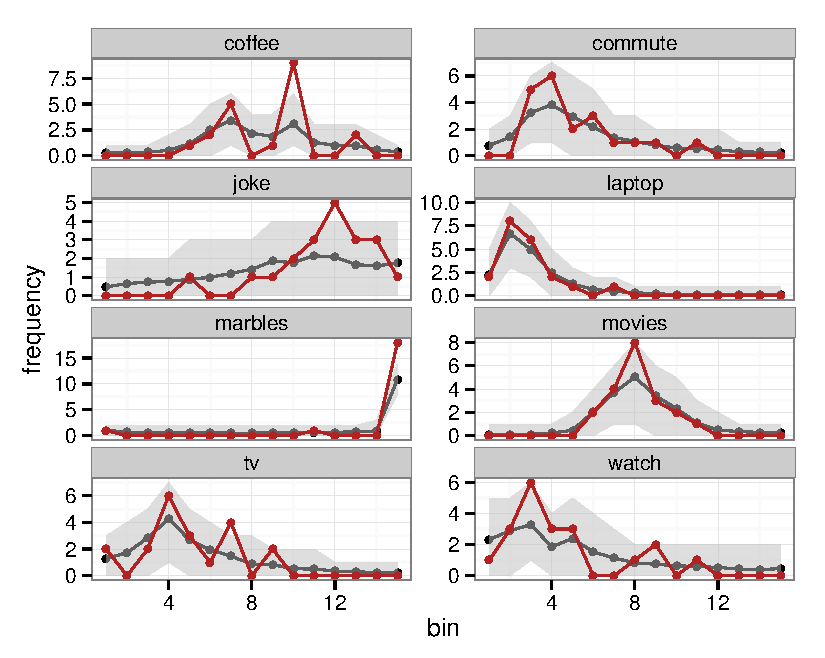
\includegraphics[width = \textwidth]{plots/ppc_number.pdf}
    \caption{number estimation}
    \label{fig:numberPPC}
  \end{subfigure}

  \begin{subfigure}[b]{0.5\textwidth}
    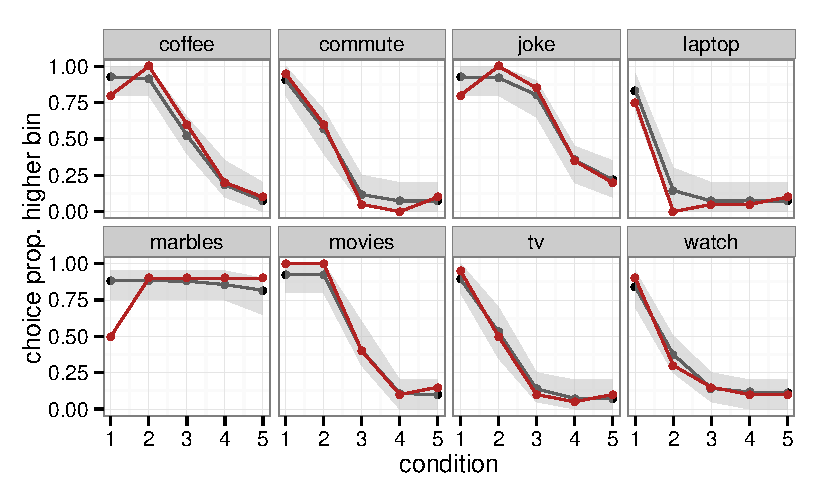
\includegraphics[width = \textwidth]{plots/ppc_choice.pdf}
    \caption{bin comparison}
    \label{fig:lightingPPC}
  \end{subfigure}

  \caption{Posterior predictive checks for aggregate data. Red lines give empirical
    observations. Black lines are means of posterior predictive samples, gray areas are
    95\% HDIs.}
  \label{fig:PPCs}
\end{figure}

Posterior predictive checks indicate that the trained model captures patterns of answers at the
aggregate population level well. To have a more fine-grained measure of model fit, we also
looked at posterior predictive $p$-values at the level of subjects and items. Unfortunately,
only the slider rating task, provides enough data for such a fine-grained analysis. For the
slider rating task, fixing a subject and an item, observations and replicates are probability
vectors of length 15. In a first analysis, we used the mean of these probability vectors as a
test statistic. The minimum posterior predictive $p$-value over all 20 (subjects) times 8
(items) cases was 0.13, suggesting that the means of observed $s_{ij}$ are non-surprising to
the trained model. In a second analysis, we used entropy as a test statistic. Two cases gave
posterior predictive $p$-values lower than 0.05. These were from the two participants who gave a
very extreme slider rating for the ``marbles'' item, basically assigning all ``mass'' to the
last bin. What this suggests is that the model can cope reasonably well also with
individual-level data, but has problems accounting for ``extreme'' choices, given that the
population-level hyper-prior on $P_{ij}$ will lead to shrinkage.

\section{Conclusions}


\section{Acknowledgments}

MF's work was supported by the Institutional Strategy of the University of T̈\"{u}bingen (Deutsche
Forschungsgemeinschaft, ZUK 63) and the Priority Program XPrag.de (DFG Schwerpunktprogramm
1727). 



\bibliographystyle{apacite}

\setlength{\bibleftmargin}{.125in}
\setlength{\bibindent}{-\bibleftmargin}

\bibliography{MyRefGlobal}


\end{document}
